\chapter{Appendix: Multivalley engineering in semiconductor microcavities}

\section{Bloch theory for exciton-photon lattices}\label{AP:A1}

Here, we present details of the bare exciton-polariton dispersion calculation in the framework of the Bloch theory.
In the main text of the manuscript, we solve the eigenvalue problem of the system with Eq.~\eqref{eq:CH2_SP1}. This equation corresponds to the eigenvalue problem of the following matrix:
%
\begin{tiny}
	\begin{equation} 	\label{AP2_EqMatSM}
		\hspace*{-10mm}
		\begin{pmatrix}
			\tilde E_C( k+G)+\tilde{V}_{C}\left( 0 \right) & \tilde{V}_{C}\left( G \right) & \tilde{V}_{C}\left( 2G \right) & 0 & 0 & \Omega \\
			\tilde{V}_{C}\left( -G \right) & \tilde E_C(k) +\tilde{V}_{C}\left( 0 \right) & \tilde{V}_{C}\left( G \right) & 0 & \Omega & 0 \\
			\tilde{V}_{C}\left( -2G \right) & \tilde{V}_{C}\left( -G \right) & \tilde E_C(k-G) + \tilde{V}_{C}\left( 0 \right) & \Omega & 0 & 0 \\
			0 & 0 & \Omega & \tilde E_X(k-G) +\tilde{V}_{X}\left( 0 \right) & \tilde{V}_{X}\left( G \right) & \tilde{V}_{X}\left( 2G \right) \\
			0 & \Omega & 0 & \tilde{V}_{X}\left( -G \right) & \tilde E_X(k)+\tilde{V}_{X}\left( 0 \right) & \tilde{V}_{X}\left( G \right)\\
			\Omega & 0 & 0 & \tilde{V}_{X}\left( -2G \right) & \tilde{V}_{X}\left( -G \right) & \tilde E_X(k+G)+\tilde{V}_{X}\left( 0 \right)
		\end{pmatrix},
	\end{equation}
\end{tiny}
%
where ${\tilde{E}_C(q)}=\frac{\hbar^2q^2}{2m_C}-\frac{i\hbar}{\tau}$ and ${\tilde{E}_X(q)}=\frac{\hbar^2q^2}{2m_X}-\frac{i\hbar}{\lambda}$. Then, $\tilde{V}_C\left( 0,-G,G \right)$ are the 0th, --1st, and 1st order terms of the Fourier series for the periodic potential of the cavity photon, and $\tilde{V}_X\left( 0,-G,G \right)$ are the 0th, --1st, and 1st order terms of the Fourier series for the excitonic potential. 
The matrix in Eq.~\eqref{AP2_EqMatSM} is reduced to the summation of terms in Eq.~\eqref{eq:CH2_SP1} from $-G$ to $G$. In our real calculations, we did the summation over the terms from $-150\cdot G$ to $150\cdot G$.

%--------------------------------------------------------------------------------------------------------

\section{Simplified model of equilibrium polariton condensation}\label{AP:A2}

Following Eqs.~\eqref{eq:CH2_H-2} and~\eqref{eq:CH2_E-2}, for the case of a fixed number of particles and low temperature, we can write the probability of occupation of different modes, referred to as the probability distribution function (PDF), as
%
\begin{equation}
	p\left( n_1, n_2 \right)=\frac{1}{\mathcal{Z}}e^{-E\left( n_1,n_2 \right)/k_B T},
	\label{AP2_ProD}
\end{equation}
%
where $\mathcal{Z}=\sum_{n_1,n_2}e^{-E\left( n_1,n_2 \right)/k_B T}$ is the partition function, $T$ is the temperature, and $k_B$ is Boltzmann's constant. The second-order correlation function then reads
%
\begin{equation}
	g_{12}^{(2)} =\frac{\langle \hat{a}_1^\dag \hat{a}_2^\dag \hat{a}_1 \hat{a}_2 \rangle}{\langle \hat{a}_1^\dag \hat{a}_1 \rangle \langle \hat{a}_2^\dag \hat{a}_2 \rangle} = \frac{\langle n_1 n_2 \rangle}{\langle n_1 \rangle \langle n_2 \rangle},
	\label{AP2_G_2}
\end{equation}

where $\langle n_1\rangle$, $\langle n_2\rangle$, and $\langle n_1n_2\rangle$ can be calculated from the PDF $p(n_1,n_2)$, see Fig.~\ref{fig:CH2_TMFig}. 
At zero temperature, $g_{12}^{(2)}=0$, confirming our earlier arguments on the choice of the state required for energy minimisation. 
With increasing temperature, $g_{12}^{(2)}$ rises as the system may be excited out of the ground state.

Allowing for the population of many modes in reciprocal space (instead of the two that we considered), the probability of occupation of any quantum state can be found by a straightforward generalisation of Eq.~\eqref{AP2_ProD}; 
in principle, the full exciton-polariton intensity distribution can then be obtained by summing over the PDF. However, in practice, the size of the Hilbert space grows exponentially with the number of particles in the system, and therefore it becomes possible to use our simple treatment to evaluate the equilibrium photoluminescence spectrum in the low-density regime with only a few particles in the system (see inset in Fig.~\ref{fig:CH2_TMFig}). 
The spectrum here was phenomenologically broadened in both energy and wave vector, accounting for the finite lifetime of the polaritons and the finite size of a typical condensate, respectively.

%--------------------------------------------------------------------------------------------------------

% \section{Entanglement Generation}\label{AP:A3}
% Here we present details on entanglement generation. We treat particles localised at the dispersion minima as two quantum modes, for which deterministic evolution is governed by the Hamiltonian in~Eq.~\eqref{eq:CH2_Hres}.
% The last term there, ${\cal \hat H}_{CK}'=4\alpha\hat a_1^\dag \hat a_2^\dag {{\hat a}_2}{{\hat a}_1}$, is a typical cross-Kerr interaction term that can be linearised by expanding the total quantum fields as $\hat a_j \rightarrow \xi_j+\delta\hat a_j$, where $\delta\hat a_j$ are displaced quantum fluctuation fields on top of classical mean fields $\xi_j$. 
% Using such a substitution and keeping terms up to the second order in $\delta \hat a_j$ only, we come up with the linearised interaction term,
% %
% \begin{eqnarray}
% 	\label{AP2_HCKlin}
% 	{\cal \hat H}_{CK}^{'\rm (lin)} &=& 4\alpha %\begin{gathered}
% 		\sum\limits_{j = 1,2} {\left[ {{{\tilde E}_j}\delta\hat a_j^\dag {\delta{\hat a}_j} + {{\tilde F}_j}( {\delta\hat a_j^\dag  + \delta{{\hat a}_j}} )} \right]} + \alpha{\cal S} \left( {\delta\hat a_1^\dag \delta\hat a_2^\dag  + {\delta{\hat a}_1}\delta{{\hat a}_2}} \right), \hfill
% 	%\end{gathered}  ,
% \end{eqnarray}

% where we assumed $\xi_{1,2}\in\mathbb{R}$ for clarity and defined ${{\tilde E}_{1,2}} = \Delta_{2,1}{\left| {{\xi _{1,2}}} \right|^2}$, ${{\tilde F}_{1,2}} = {\xi _{1,2}}{\left| {{\xi _{2,1}}} \right|^2}$ and ${\cal S}=\xi_1\xi_2$.
% The first term is an energy shift, the second is an effective driving term, and crucially, the last term is the typical two-mode squeezing interaction of magnitude ${\cal S}$ set by the product of the two mean fields $\xi_{1,2}$, and is thus responsible for the entanglement between the two modes.
% The squeezing and entanglement magnitude can therefore be adjusted by varying the resonant driving strengths, $F_{1,2}$.

%--------------------------------------------------------------------------------------------------------

\section{Nonequilibrium model of polariton condensation}\label{AP:A4}
Now we present details on the nonequilibrium model.
Interaction with the reservoir of acoustic phonons in a semiconductor crystal lattice is described by the microscopic Fr\"ohlich Hamiltonian~\cite{Tassone:1997aa}:
%
\begin{eqnarray}
	\hat{\mathcal{H}}_\textrm{int}=\sum_{\mathbf{q},k}G_{\mathbf{q}}\hat{b}_{\mathbf{q}}\hat{a}^\dagger_{k+q_x}
	\hat{a}_k+G_{\mathbf{q}}^*\hat{b}^\dagger_{\mathbf{q}}\hat{a}_{k+q_x}\hat{a}^\dagger_k,
	\label{AP2_neq}
\end{eqnarray}

where parameters $G_{\mathbf{q}}$ are the exciton--phonon interaction strengths evaluated elsewhere~\cite{Hartwell:2010aa}.
The phonon wavevector here is
$\mathbf{q}=\mathbf{e}_xq_x+\mathbf{e}_yq_x+\mathbf{e}_zq_z$, where $\mathbf{e}_x$,
$\mathbf{e}_y$, and $\mathbf{e}_z$ are unit vectors: $\mathbf{e}_x$ is in the direction of the 1D polariton system, $\mathbf{e}_z$ is in the structure growth direction, and $\mathbf{e}_y$ is perpendicular to both.
%
The phonon dispersion relation, $\hbar\omega_{\mathbf{q}}=\hbar
c_s\sqrt{q_x^2+q_y^2+q_z^2}$, is determined by the sound velocity, $c_s$.

The equations of motion for the polariton macroscopic wavefunction, $\psi$, and the exciton reservoir occupation number, $n_\textrm{R}$, read~\cite{Savenko:2013aa,Wouters:2007aa}:
%
\begin{eqnarray}
	\label{AP2_EqGPEnR}
	&&i\hbar\frac{\partial\psi(x,t)}{\partial t}={\cal F}^{-1}\left[E_k\psi_k+{\cal S}_k(t)\right] +\frac{i\hbar}{2}\left[Rn_\textrm{R}(x,t)-\gamma_0-\frac{2i}{\hbar}\alpha|\psi({x},t)|^2\right]\psi(x,t)\nonumber \\
	&&~~~~~~~~~~~~~~~~~~  +\sum_k\left[{\cal T}_{-k}(t)+{\cal T}^*_k(t)\right]e^{-ikx}\psi(x,t);\\
	\label{AP2_EqGPEnR2}
	&&\frac{\partial n_\textrm{R}(x,t)}{\partial t}=-(\gamma_\textrm{R}+R|\psi(x,t)|^2)n_\textrm{R}+P,
\end{eqnarray}
%
where ${\cal F}^{-1}$ stands for the inverse Fourier transform, $E_k$ is the free polariton dispersion, $\psi_k$ is the Fourier image of the macroscopic wavefunction, $P$ and $\gamma_\textrm{R}$ are the incoherent reservoir homogeneous pumping intensity and inverse lifetime of the reservoir, respectively, and $R$ is the system-reservoir excitation exchange rate.
The term ${\cal S}_k(t)$ corresponds to the emission of phonons by a condensate stimulated by polariton concentration.

The stochastic term ${\cal T}_{q_x}$ in the last line of Eq.~\eqref{AP2_EqGPEnR} is defined by the correlations:
%
\begin{align}
	\left<{\cal T}_{q_x}^*(t){\cal T}_{q_x^\prime}(t^\prime)\right>&=\sum_{q_y,q_y}\left|G_{{q_x,q_y,q_z}}\right|^2n_{q_x,q_y,q_z}\delta_{q_x,q_x^\prime}\delta(t-t^\prime);\notag\\
	\left<{\cal T}_{q_x}(t){\cal T}_{q_x^\prime}(t^\prime)\right>&=
	\left<{\cal T}_{q_x}^*(t){\cal T}_{q_x^\prime}^*(t^\prime)\right>=0,
	\label{AP2_EqThermal}
\end{align}
%
where $n_{\mathbf{q}}$ is the temperature-dependent density of phonons in the state with wavevector $\mathbf{q}$.

Solving Eq.~\eqref{AP2_EqGPEnR} numerically and averaging over different stochastic realizations of the phonon field, we obtained the result shown in Fig.~\ref{fig:CH2_Fig4} of the main text.

%--------------------------------------------------------------

\section{Energy Band Structure}\label{AP:A5}
Here we discuss the energy band structure of the exciton-polariton lattice [Fig.~\ref{fig:CH2_Fig1}(a)] as well as an alternative configuration.
%
%
%
\begin{figure}[ht]
	\centering
	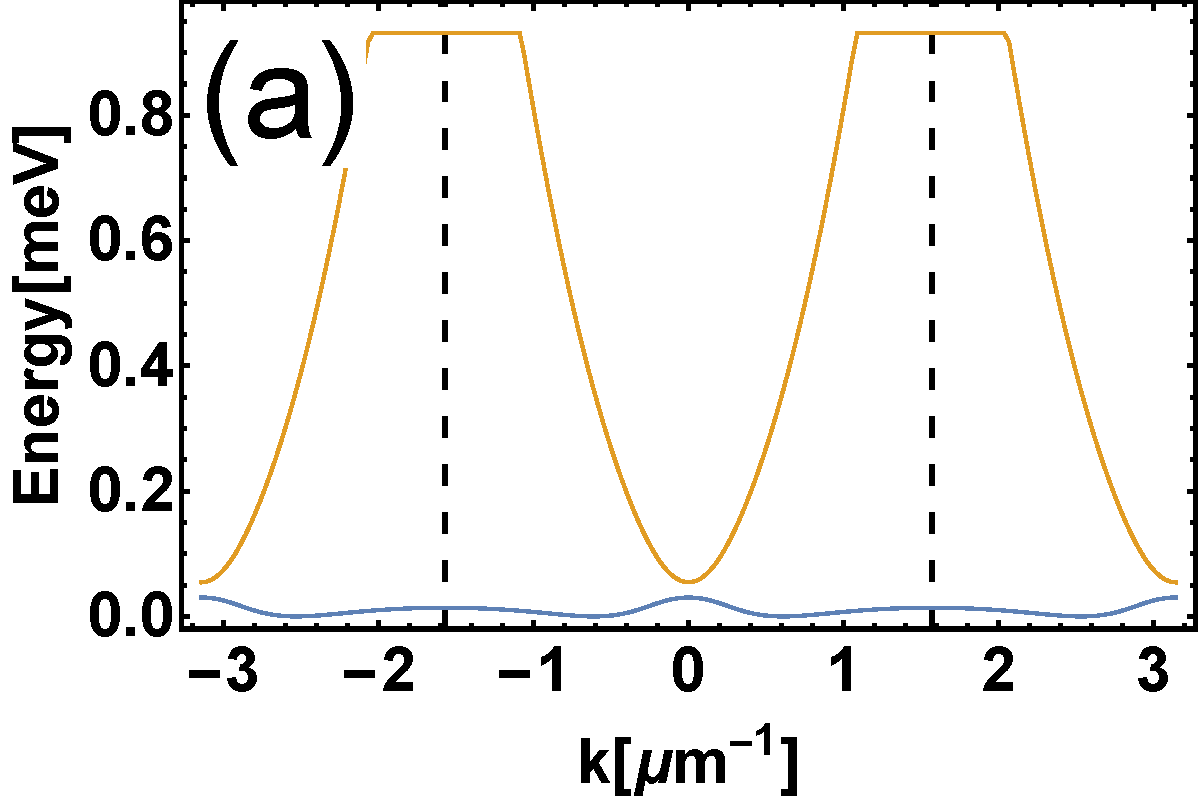
\includegraphics[width=0.45\linewidth]{Fig/Ap2/SP-1.pdf}
	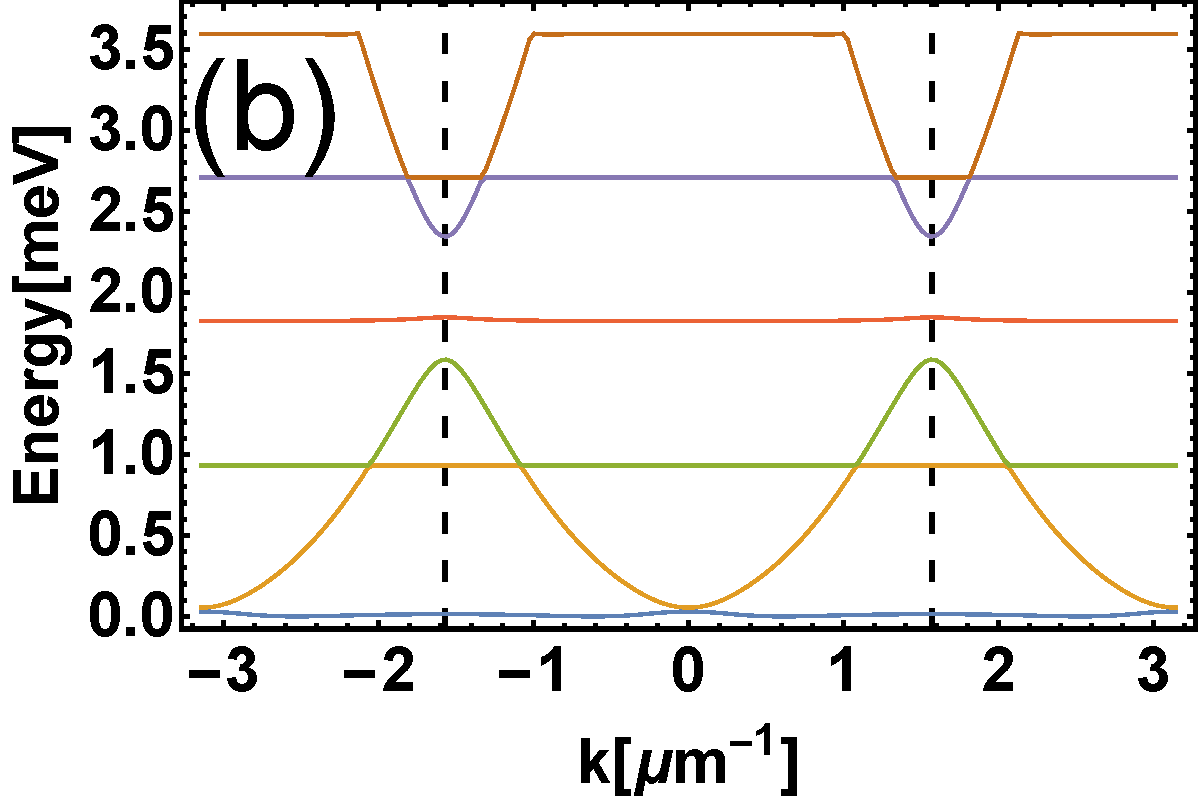
\includegraphics[width=0.45\linewidth]{Fig/Ap2/SP-2.pdf}
	\caption[Band spectrum]{Energy bands in (a) level 1 and level 2, and from (b) level 1 to level 6.  Picture from \cite{Sun:2017ab}.}
	\label{fig:AP2_s-1}
\end{figure}
%
%
%
%
%
%
\begin{figure}[ht]
	\centering
	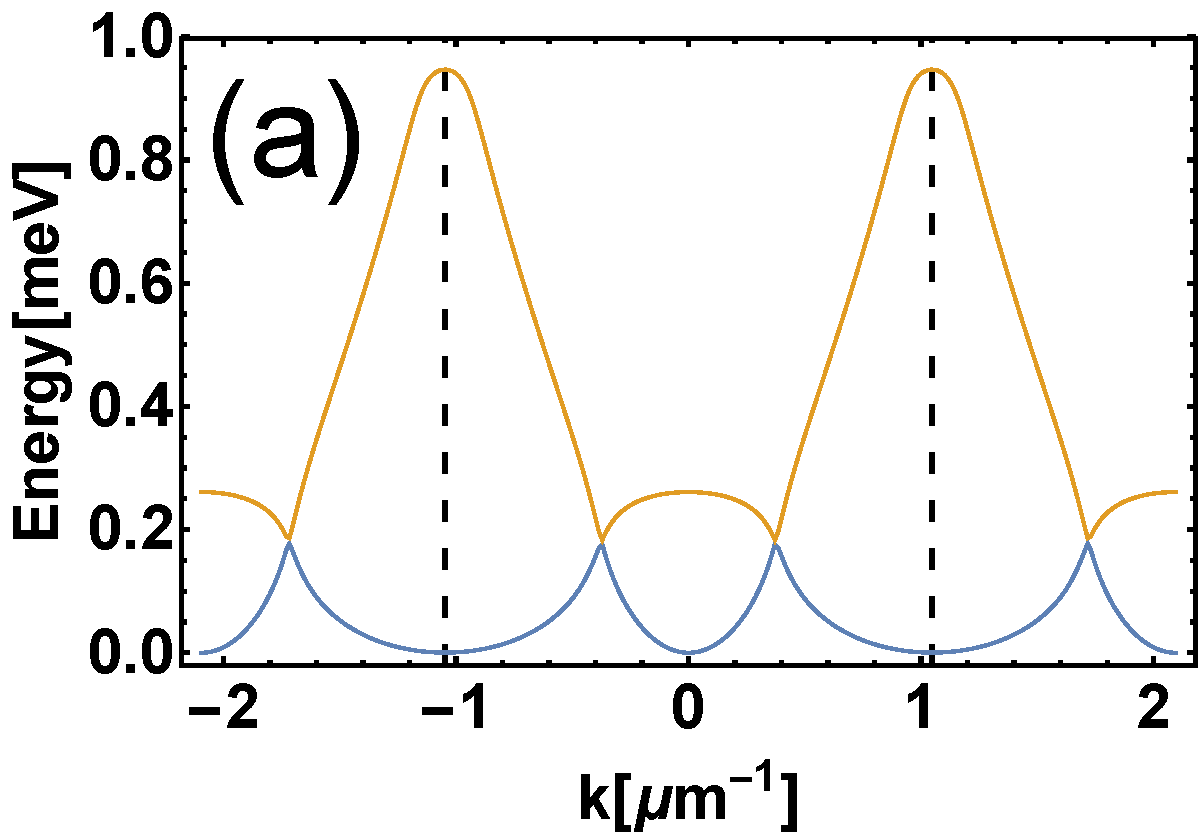
\includegraphics[width=0.45\linewidth]{Fig/Ap2/SP-3.pdf}
	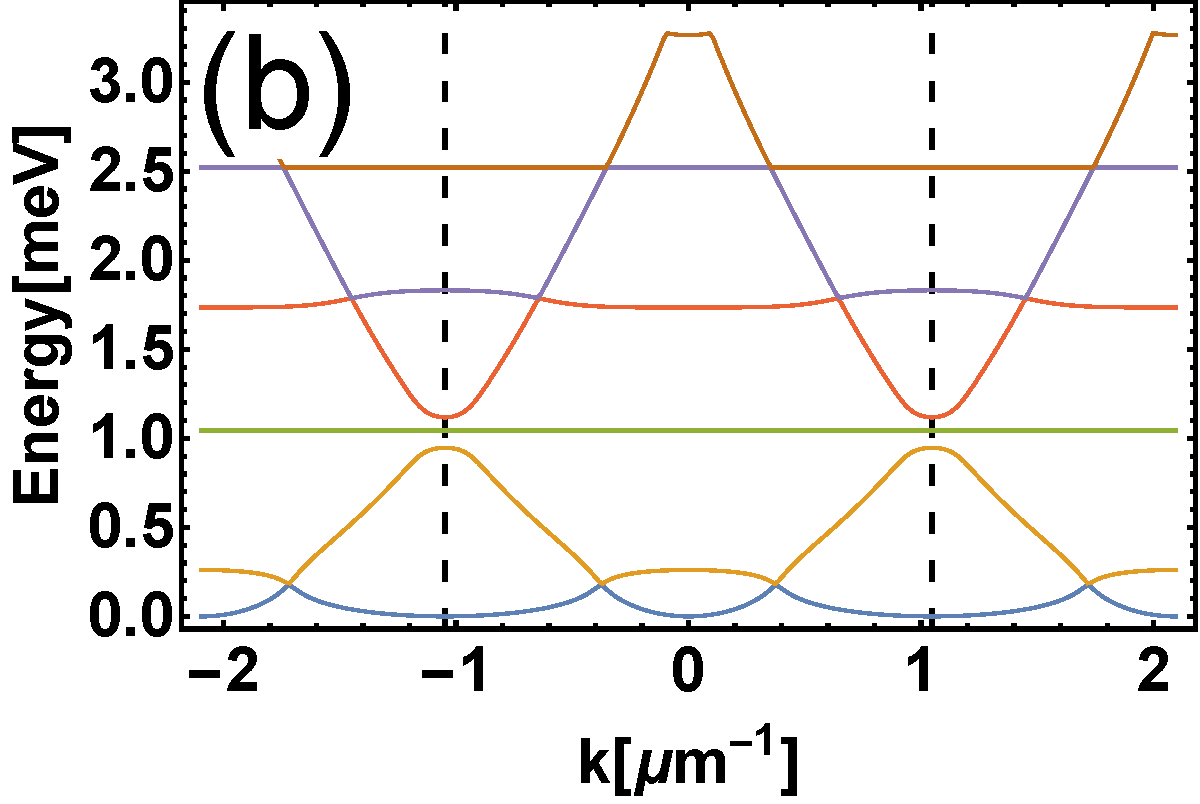
\includegraphics[width=0.45\linewidth]{Fig/Ap2/SP-4.pdf}
	\caption[Band spectrum in the alternative configuration ]{Energy bands in the case where the minima in $k$-space are at the $\Gamma$ point and the edge of the Brillouin zone, for (a) level 1 and level 2 bands, and (b) level 1 to level 6 bands. The figure is taken from~\cite{Sun:2017ab}.}
	\label{fig:AP2_s-2}
\end{figure}
%
%
%
The parameters for these plots are as follows. Lattice period: $T=2.0$ $\mu$m; potential profile for the cavity photons: sine function $-1.1\sim0.25$ meV; potential profile for the excitons: sine function $-0.95 \sim 460.29$ meV; exciton-photon coupling constant: $\Omega=0.7$ meV; decay rate of the cavity photons: $\gamma =0.42$ meV; decay rate of the excitons: $0.04 $ meV; effective mass of a cavity photon: $5*10^{-5} m_e$; effective mass of an exciton: $0.22 m_e$, where $m_e$ is the free electron mass.

Let us also change the parameters of the potential energies of the excitons and photons to see which dispersion we can achieve in $k$-space.
%
%
%
\begin{figure}[ht]
	\centering
	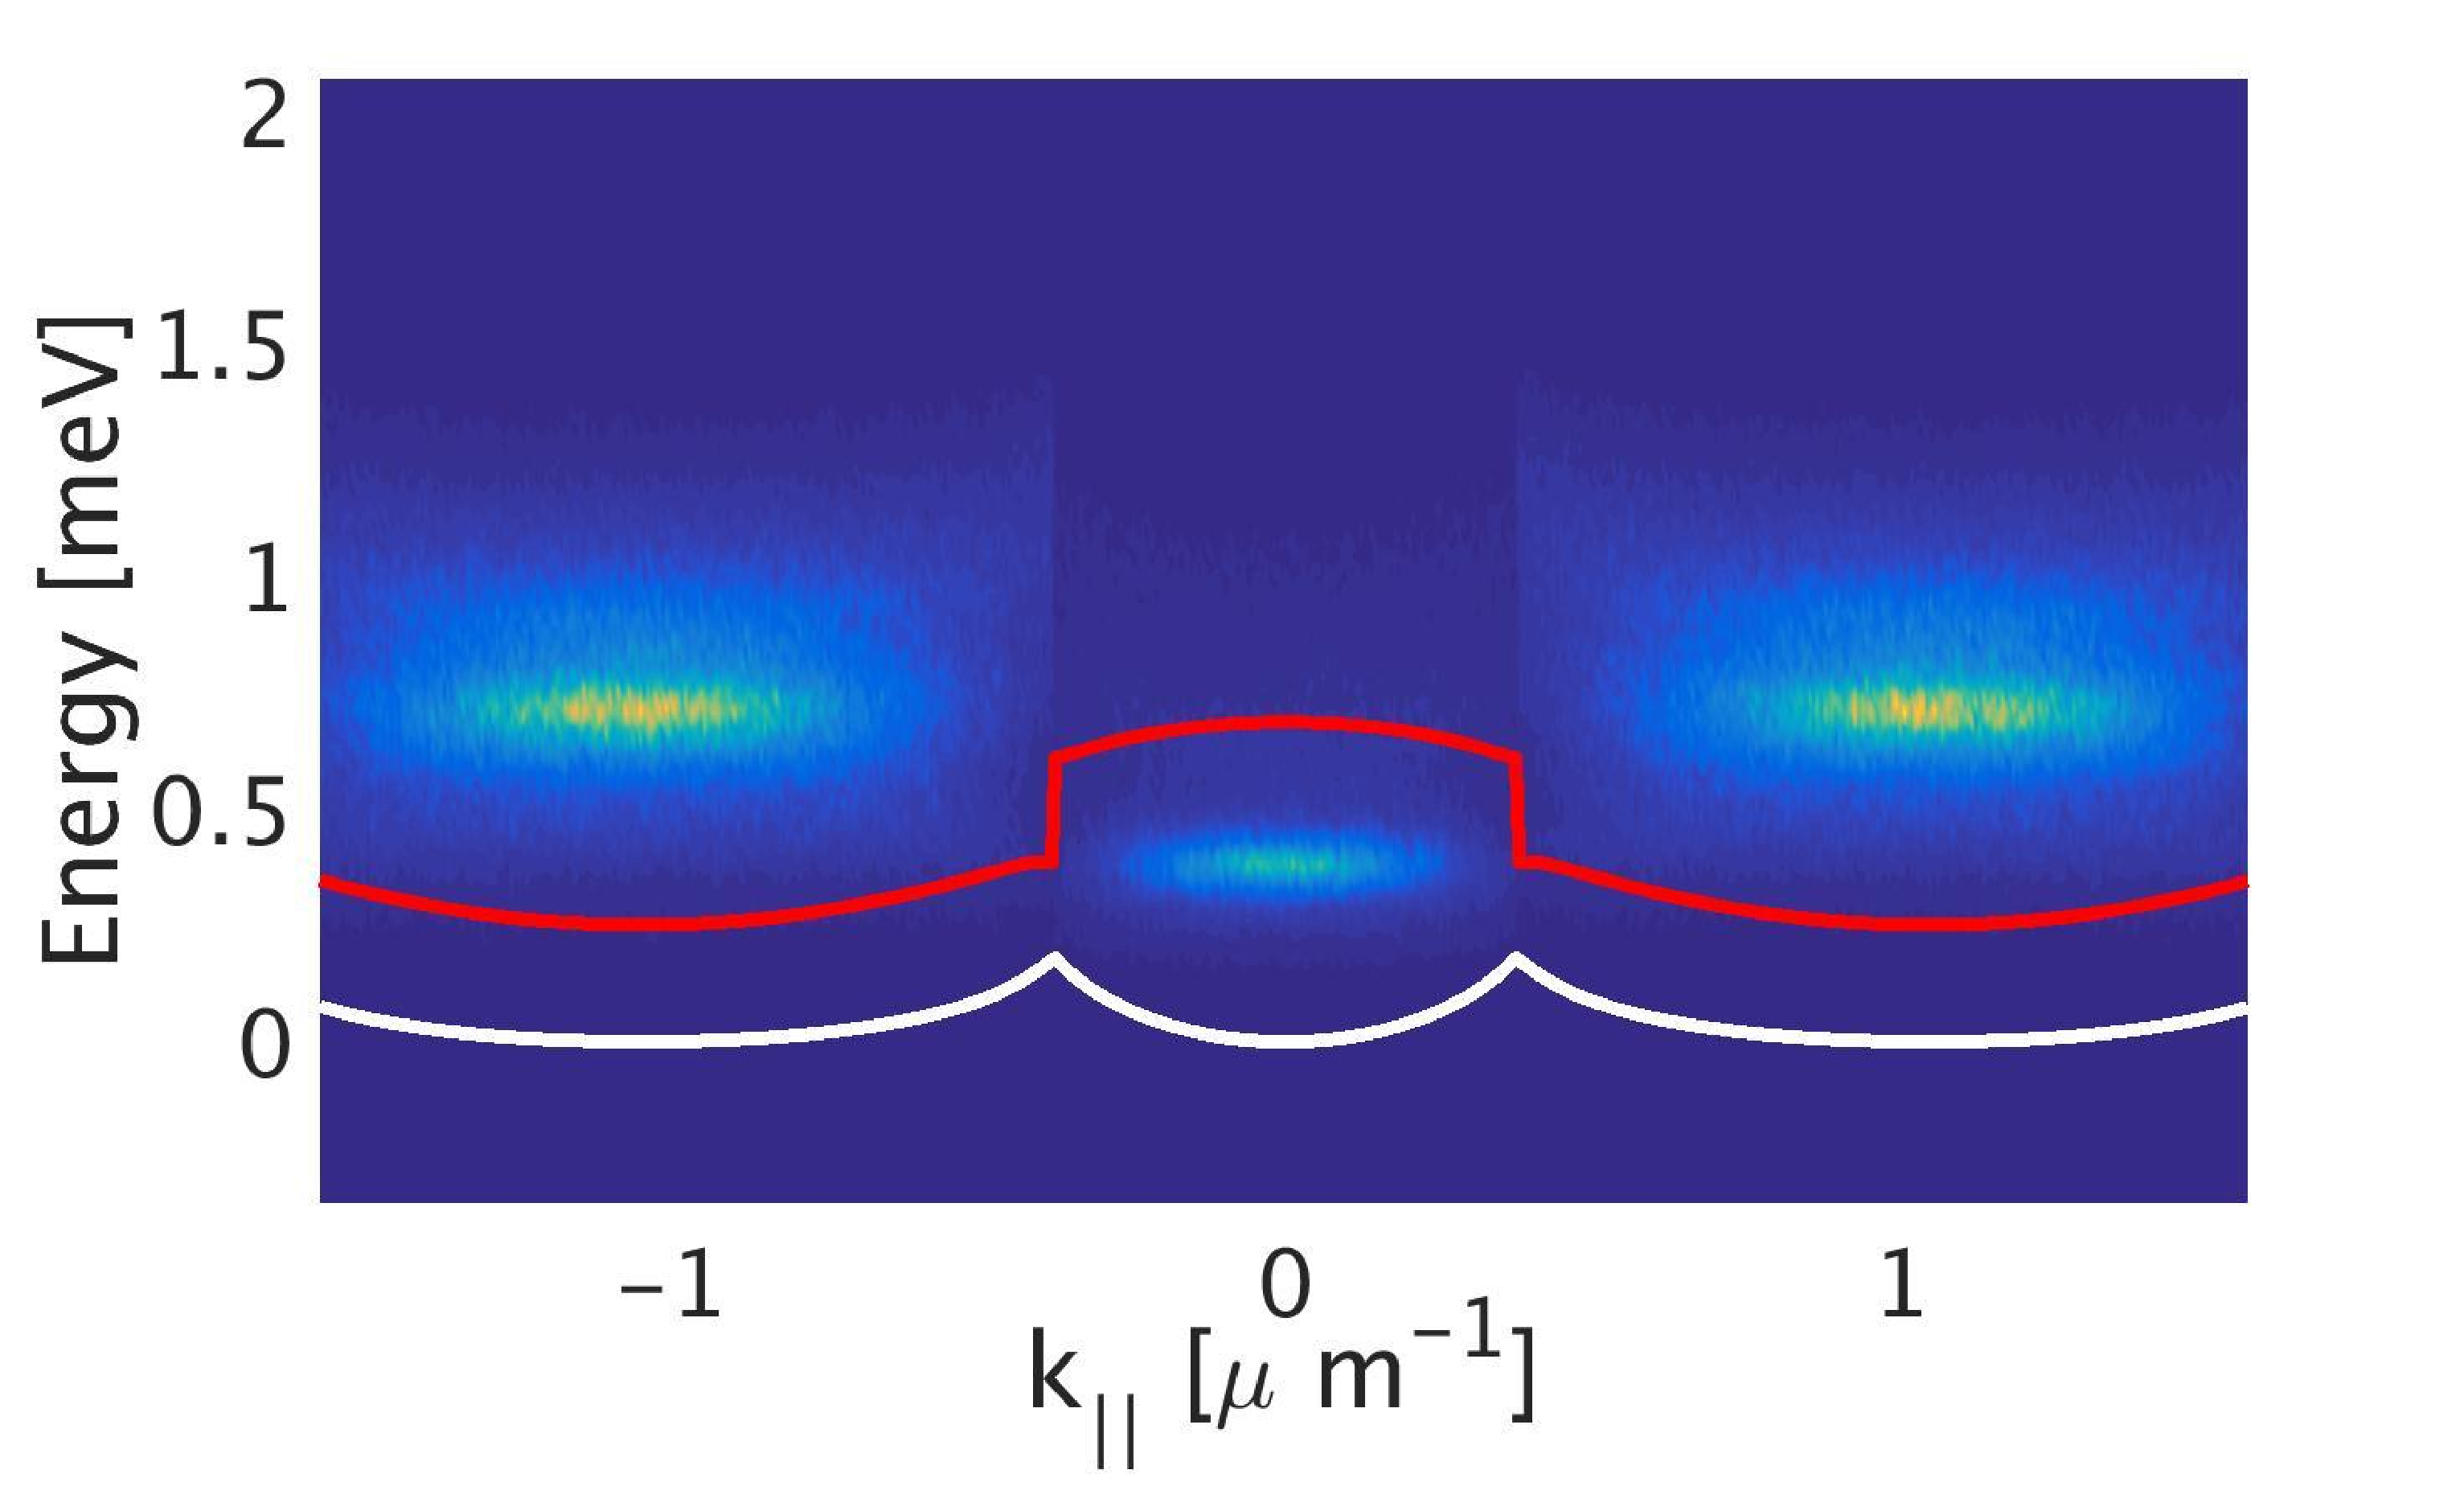
\includegraphics[width=0.555555\linewidth]{Fig/Ap2/SP-5.pdf}
	\caption[Condensation in the alternative configuration]{Condensate result from the energy dispersion in Fig.~\ref{fig:AP2_s-2}. The red and white lines represent the decay rate and the energy dispersion of the polariton, respectively. The figure is taken from~\cite{Sun:2017ab}.}
	\label{fig:AP2_s-3}
\end{figure}
%
%
%
By taking the following parameters, we yield the dispersion presented in Figs.~\ref{fig:AP2_s-2} and~\ref{fig:AP2_s-3}. Lattice period: $T=3.0$ $\mu$ m; potential profile for the cavity photons: square function $-0.25\sim0$ meV; potential profile for the excitons: sine function $-0.389 \sim 697.95$ meV; exciton-photon coupling constant: $\Omega=2.47$ meV; decay rate of the cavity photons: $\gamma =1$ meV; decay rate of the excitons: $0$ meV, effective mass of a cavity photon: $5*10^{-5} m_e$; effective mass of an exciton: $0.22 m_e$.

Figure~\ref{fig:AP2_s-3} is the result of the nonequilibrium model. Since the decay rate of the exciton-polaritons varies significantly with momentum $k$, it becomes easier for exciton-polaritons to condense at $k=\pm k_{BZ}$ rather than at $k=0$. As a result, the blueshifts differ at $k=0$ and $k=\pm k_{BZ}$. The minima in $k$-space become inequivalent in properties, making it difficult to consider entanglement between them. It should be noted, though, that the two minima at $k=\pm k_0$ in Fig.~\ref{fig:CH2_Fig4}(b) are equivalent in properties.


Figure~\ref{fig:AP2_s-4} is a 3D plot of the energy dispersion in the 2D lattice corresponding to Fig.~\ref{fig:CH2_Fig2D}(a).

\begin{figure}[!tb]
\centering
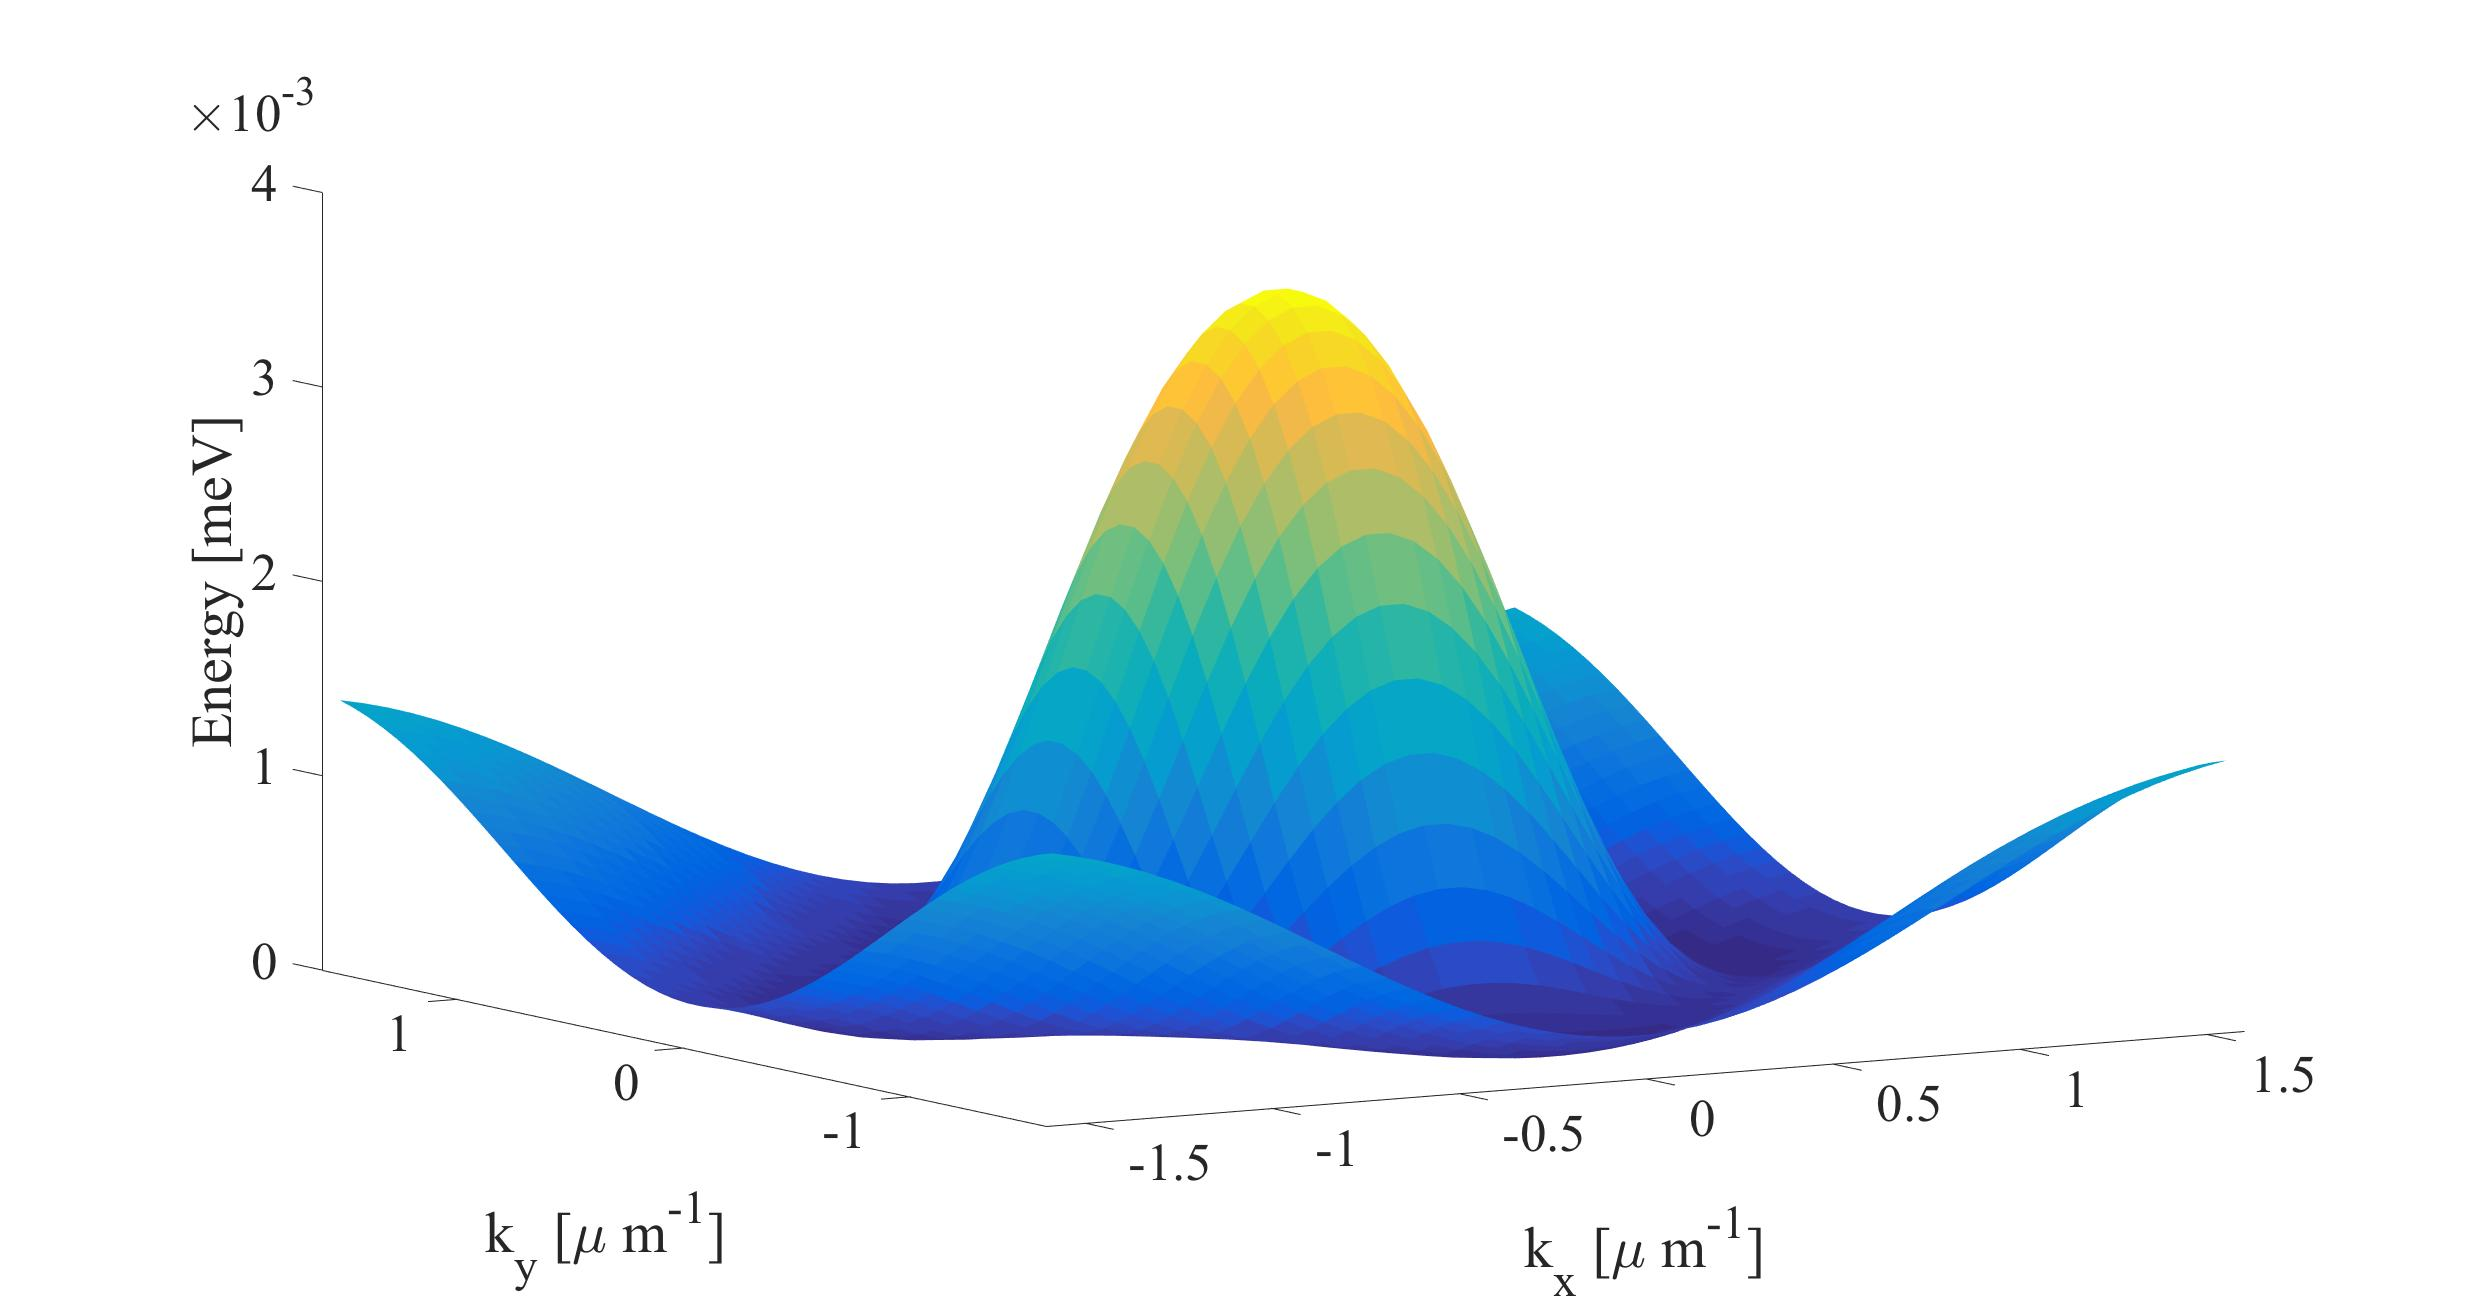
\includegraphics[height=0.4\linewidth]{Fig/Ap2/Bands_surf.jpg}
\caption[Ground state dispersion in 3D]{Energy dispersion in the 2D lattice. The figure is taken from~\cite{Sun:2017ab}.}
\label{fig:AP2_s-4}
\end{figure}
